\documentclass[a4paper,12pt]{article} % тип документа

% Поля страниц
\usepackage[left=2.5cm,right=2.5cm,
    top=2cm,bottom=2cm,bindingoffset=0cm]{geometry}
 
    
%Отступ после заголовка    
\usepackage{indentfirst}


% Рисунки
\usepackage{floatrow,graphicx,calc}
\usepackage{wrapfig}

% Создаёем новый разделитель
\DeclareFloatSeparators{mysep}{\hspace{1cm}}

% Ссылки?
\usepackage{hyperref}
\usepackage[rgb]{xcolor}
\hypersetup{				% Гиперссылки
    colorlinks=true,       	% false: ссылки в рамках
	urlcolor=blue          % на URL
}


%  Русский язык
\usepackage[T2A]{fontenc}			% кодировка
\usepackage[utf8]{inputenc}			% кодировка исходного текста
\usepackage[english,russian]{babel}	% локализация и переносы


% Математика
\usepackage{amsmath,amsfonts,amssymb,amsthm,mathtools}


% Что-то 
\usepackage{wasysym}

\begin {document}

\begin{titlepage}
\newcommand{\HRule}{\rule{\linewidth}{0.3 mm}} % Defines a Hnew command for the horizontal lines, change thickness here

\center % Center everything on the page
 
%----------------------------------------------------------------------------------------
%	HEADING SECTIONS
%----------------------------------------------------------------------------------------

\textsc{\Large Московский физико-технический институт }\\[1.5cm] % Name of your university/college
\textsc{\Large Факультет аэрокосмических технологий}\\[0.5cm] % Major heading such as course name
\textsc{\large Лабораторная работа 2.2.3}\\[0.5cm] % Minor heading such as course title

%----------------------------------------------------------------------------------------
%	TITLE SECTION
%----------------------------------------------------------------------------------------

\HRule \\[0.4cm]
{ \huge \bfseries Измерение теплопроводности воздуха при атмосферном давлении }\\[0.4cm] % Title of your document
\HRule \\[1.5cm]
 
%----------------------------------------------------------------------------------------
%	AUTHOR SECTION
%----------------------------------------------------------------------------------------

\begin{minipage}{0.4\textwidth}
\begin{flushleft} \large
\emph{Автор:}\\ Артем \textsc{Овчинников} % Your name
\end{flushleft}
\end{minipage}
\begin{minipage}{0.4\textwidth}
\begin{flushright} \large
\emph{Преподаватель:} \\
Арина Владимировна \textsc{Радивон} % Supervisor's Name
\end{flushright}
\end{minipage}\\[4cm]
%	DATE SECTION
%----------------------------------------------------------------------------------------

{\large \today}\\[2cm] % Date, change the \today to a set date if you want to be precise

%----------------------------------------------------------------------------------------
%	LOGO SECTION
%----------------------------------------------------------------------------------------

 
%----------------------------------------------------------------------------------------

\vfill % Fill the rest of the page with whitespace

\end{titlepage}
\tableofcontents
\newpage
\section{Аннотация}
В работе представлено измерение коэффициента теплопроводности воздуха при атмосферном давлении в зависимости от температуры.
\section{Теоретические сведения}
Теплопроводность — это процесс передачи тепловой энергии от нагретых частей системы к холодным за счёт хаотического движения частиц среды (молекул, атомов и т.п.). \\
Перенос тепла описывается законом Фурье, утверждающим, что плотность потока энергии (количество теплоты, переносимое через единичную площадку в единицу времени) пропорциональна градиенту температуры:
\begin{equation}
    \Vec{q} = -k \cdot \nabla T
\end{equation}
где к — коэффициент теплопроводности. \\
В цилиндрически симметричной установке, в которой тепловой поток направлен к стенкам цилиндра от нити, полынй поток тепла $Q = qS$ через каждую цилиндрическую поверхность радиуса $r$ должен в стационарном состоянии быть неизменен (как в пространстве, так и во времени). Тогда
\begin{equation}
	Q = -2\pi rL\varkappa \frac{dT}{dr} = const,	
\end{equation}
откуда получаем формулу
\begin{equation}
	\label{formula}
	T_1 - T_2 = \frac{Q}{2\pi L\varkappa} \ln \frac{r_2}{r_1}.
\end{equation}
Здесь $r_1$ и $T_1$ -- радиус и температура нити, $r_2$ и $T_2$ -- радиус и температура цилиндра.

\thisfloatsetup{floatrowsep=mysep}	
\begin{figure}[h!]
\begin{floatrow}
 \ffigbox[\FBwidth]{\caption{теоретическая модель}\label{fig:Graph_5}}%
         {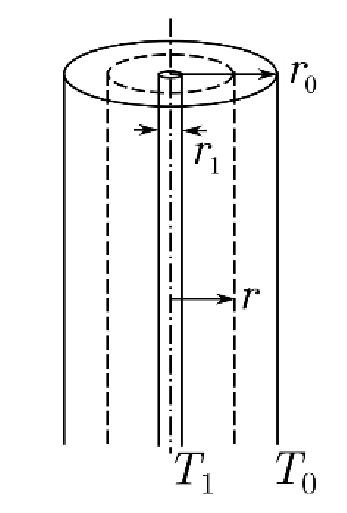
\includegraphics[width=7cm,height=7.875cm]{physlabwork_11week_th.png}}     
\end{floatrow}
\end{figure}

\section{Методика измерений}
Принципиально неустранимая систематическая
ошибка измерения температуры с помощью термометра сопротивления возникает из-за необходимости пропускать через резистор (нить) измерительный ток. Чем этот ток выше, тем с большей точностью будет измерен как он сам,
так и напряжение. Однако при этом квадратично возрастает выделяющаяся на резисторе мощность. Следовательно, температура резистора становится меня держит в заложниках кафедра общефиза, спасите выше, чем у объекта, температуру которого надо измерить. Измерения же при малых токах не дают достаточной точности (в частности, из-за существенного вклада термоэлектрических явлений в проводниках и контактах).
Эта проблема решается построением нагрузочной кривой — зависимости измеряемого сопротивления от выделяющейся в нём мощности, с последующей экстраполяцией к нулевой мощности для определения сопро-
тивления, при котором его температура равна температуре измеряемого объекта. Кроме того, в данной работе измерение нагрузочных кривых позволяет в ходе эксперимента получить температурную зависимость сопротивления нити, так как при температура нити равна температуре термостата.
\section{Используемое оборудование}
На оси полой цилиндрической трубки размещена металлическая нить. Полость трубки заполнена воздухом (полость через небольшое отверстие сообщается с атмосферой). Стенки трубки помещены в кожух, через которых пропускается вода из термостата, так что их температура поддерживается постоянной. Для предотвращения конвекции трубка расположена вертикально.

\thisfloatsetup{floatrowsep=mysep}	
\begin{figure}[h!]
\begin{floatrow}
 \ffigbox[\FBwidth]{\caption{схема установки}\label{fig:Graph_5}}%
         {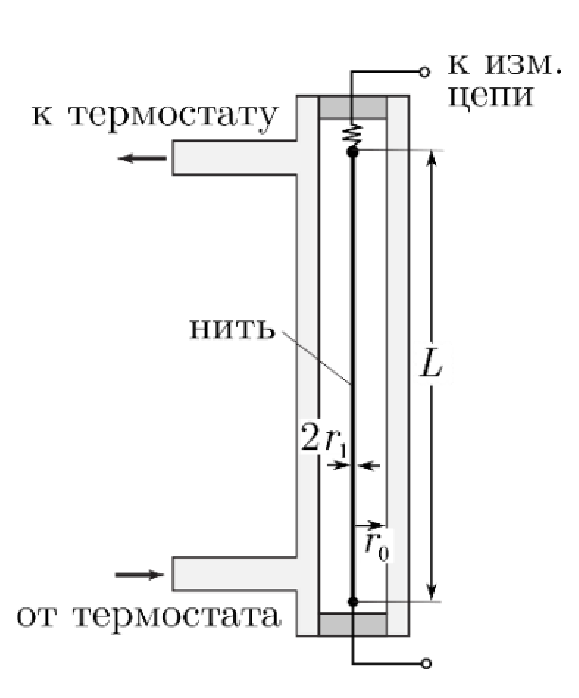
\includegraphics[width=7cm,height=7.875cm]{physlabwork_11week_set.png}}     
\end{floatrow}
\end{figure}

\newgeometry{bottom=2cm, left=1cm, right=1cm, top=1.5cm}	
\thisfloatsetup{floatrowsep=mysep}	
\begin{figure}[h!]
\begin{floatrow}
 \ffigbox[\FBwidth]{\caption{мои данные}\label{fig:Graph_1}}%
         {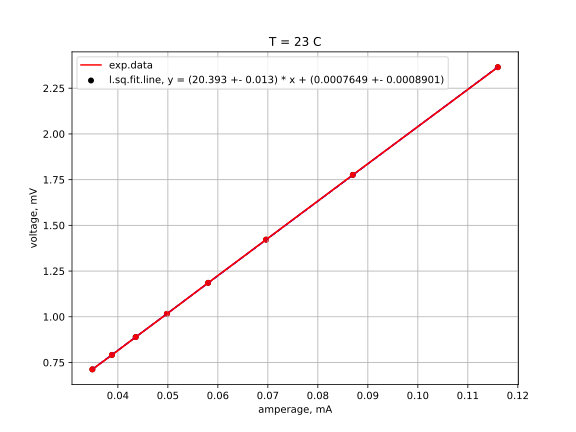
\includegraphics[width=8cm,height=7cm]{physlabwork_11week_1.png}}
 \ffigbox[\FBwidth]{\caption{мои данные}\label{fig:Graph_2}}%
         {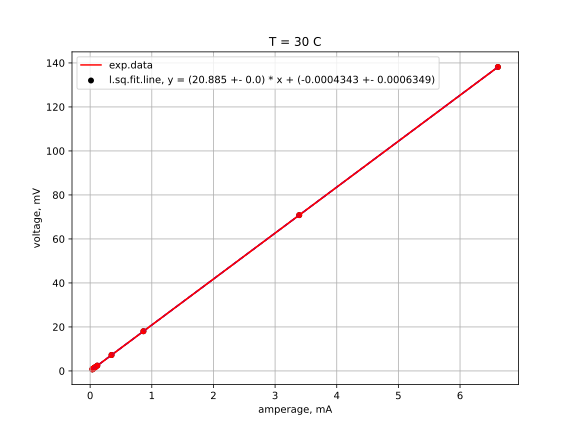
\includegraphics[width=8cm,height=7cm]{physlabwork_11week_2.png}}         
\end{floatrow}
\end{figure}

\thisfloatsetup{floatrowsep=mysep}	
\begin{figure}[h!]
\begin{floatrow}
 \ffigbox[\FBwidth]{\caption{мои данные}\label{fig:Graph_3}}%
         {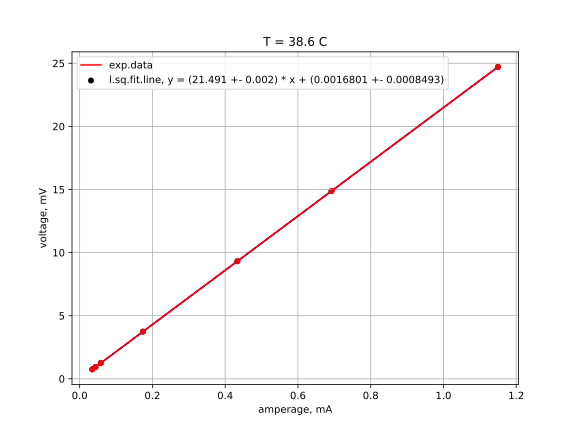
\includegraphics[width=8cm,height=7cm]{physlabwork_11week_3.png}}
 \ffigbox[\FBwidth]{\caption{мои данные}\label{fig:Graph_4}}%
         {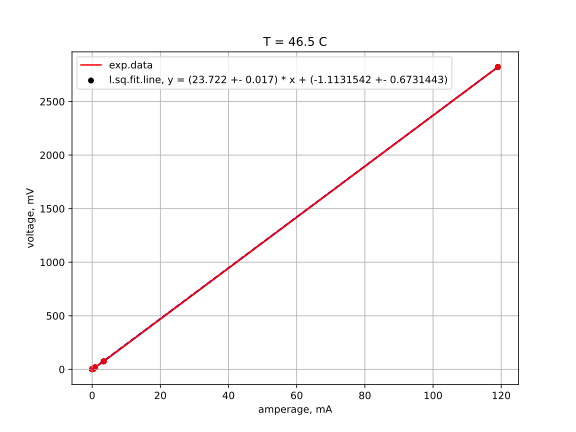
\includegraphics[width=8cm,height=7cm]{physlabwork_11week_4.png}}         
\end{floatrow}
\end{figure}

\thisfloatsetup{floatrowsep=mysep}	
\begin{figure}[h!]
\begin{floatrow}
 \ffigbox[\FBwidth]{\caption{мои данные}\label{fig:Graph_5}}%
         {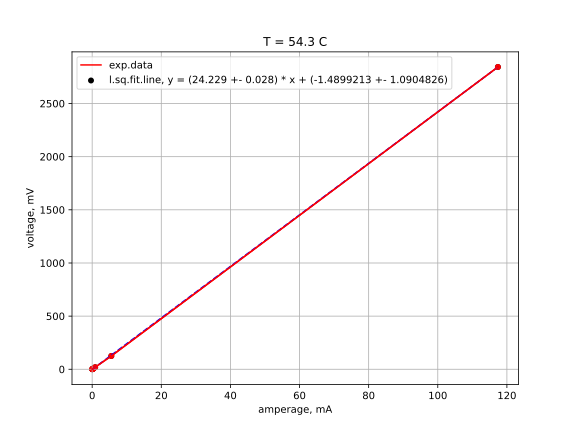
\includegraphics[width=8cm,height=7cm]{physlabwork_11week_5.png}}
 \ffigbox[\FBwidth]{\caption{мои данные}\label{fig:Graph_6}}%
         {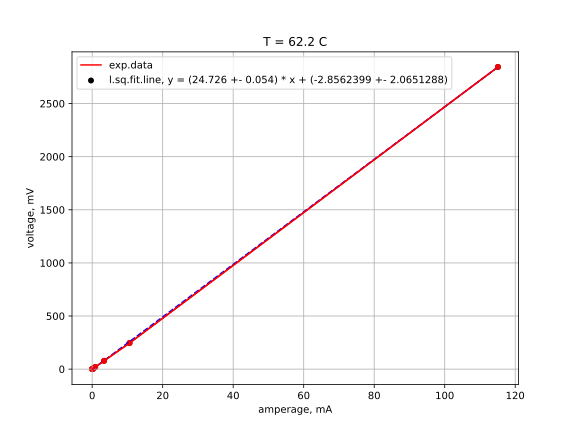
\includegraphics[width=8cm,height=7cm]{physlabwork_11week_6.png}}         
\end{floatrow}
\end{figure}
\restoregeometry

\newgeometry{bottom=2cm, left=1cm, right=1cm, top=1.5cm}	
\thisfloatsetup{floatrowsep=mysep}	
\begin{figure}[h!]
\begin{floatrow}
 \ffigbox[\FBwidth]{\caption{мои данные}\label{fig:Graph_1}}%
         {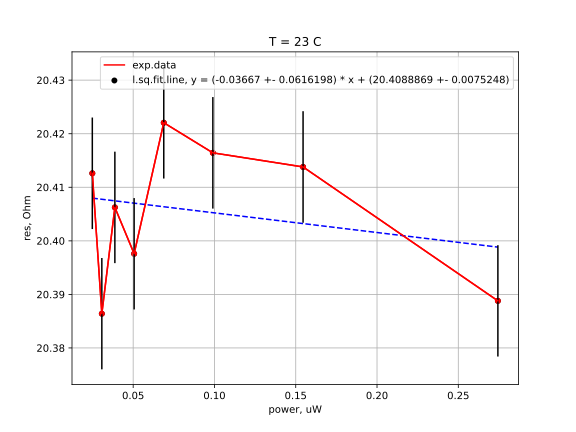
\includegraphics[width=8cm,height=7cm]{physlabwork_11week_1RQ.png}}
 \ffigbox[\FBwidth]{\caption{мои данные}\label{fig:Graph_2}}%
         {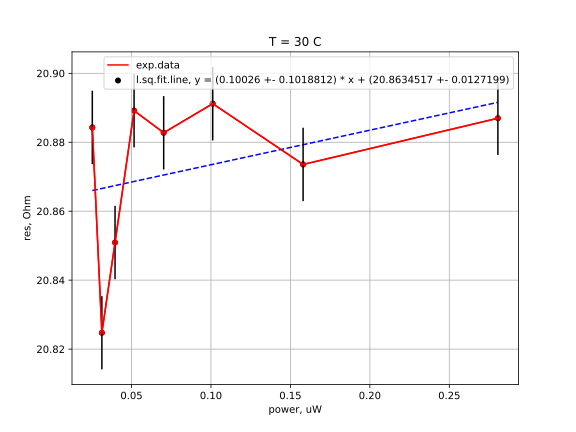
\includegraphics[width=8cm,height=7cm]{physlabwork_11week_2RQ.png}}         
\end{floatrow}
\end{figure}

\thisfloatsetup{floatrowsep=mysep}	
\begin{figure}[h!]
\begin{floatrow}
 \ffigbox[\FBwidth]{\caption{мои данные}\label{fig:Graph_3}}%
         {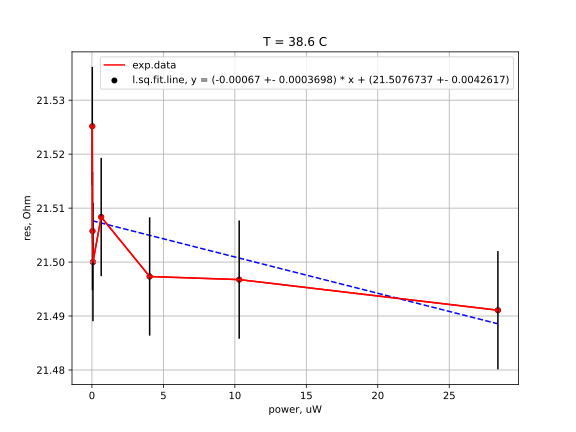
\includegraphics[width=8cm,height=7cm]{physlabwork_11week_3RQ.png}}
 \ffigbox[\FBwidth]{\caption{мои данные}\label{fig:Graph_4}}%
         {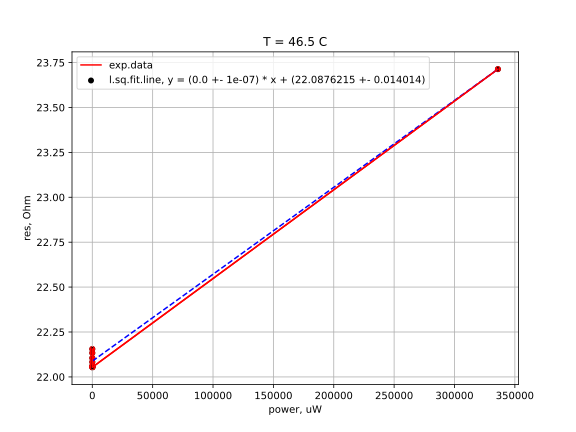
\includegraphics[width=8cm,height=7cm]{physlabwork_11week_4RQ.png}}         
\end{floatrow}
\end{figure}

\thisfloatsetup{floatrowsep=mysep}	
\begin{figure}[h!]
\begin{floatrow}
 \ffigbox[\FBwidth]{\caption{мои данные}\label{fig:Graph_5}}%
         {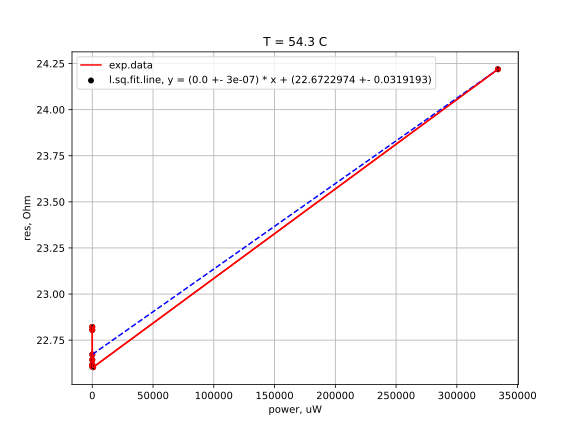
\includegraphics[width=8cm,height=7cm]{physlabwork_11week_5RQ.png}}
 \ffigbox[\FBwidth]{\caption{мои данные}\label{fig:Graph_6}}%
         {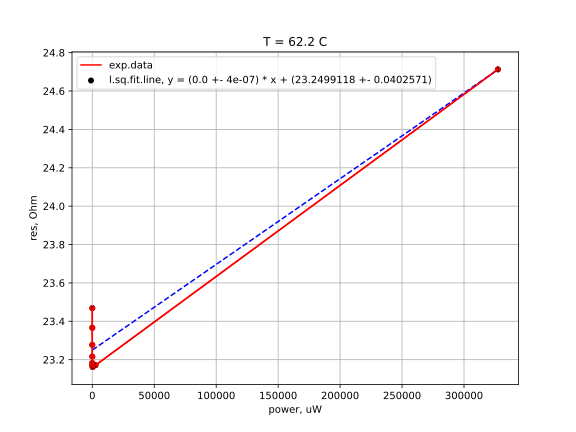
\includegraphics[width=8cm,height=7cm]{physlabwork_11week_6RQ.png}}         
\end{floatrow}
\end{figure}
\restoregeometry

\newgeometry{bottom=2cm, left=1cm, right=1cm, top=1.5cm}	
\thisfloatsetup{floatrowsep=mysep}	
\begin{figure}[h!]
\begin{floatrow}
 \ffigbox[\FBwidth]{\caption{не мои данные}\label{fig:Graph_1}}%
         {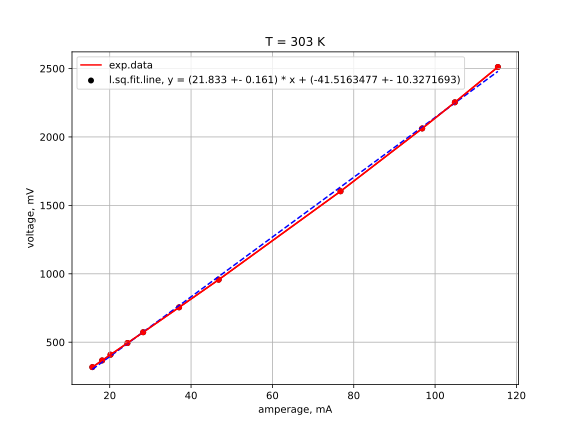
\includegraphics[width=8cm,height=7cm]{physlabwork_11week_1n.png}}
 \ffigbox[\FBwidth]{\caption{не мои данные}\label{fig:Graph_2}}%
         {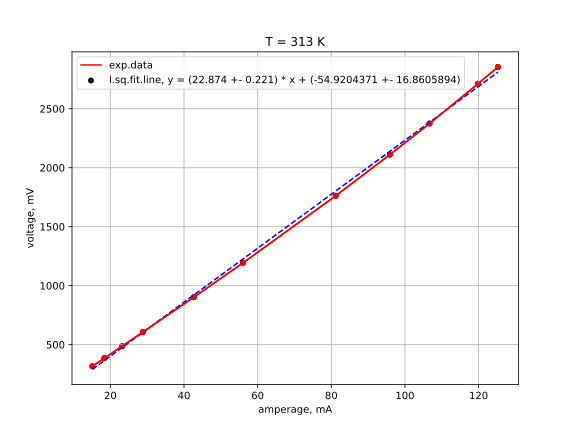
\includegraphics[width=8cm,height=7cm]{physlabwork_11week_2n.png}}         
\end{floatrow}
\end{figure}

\thisfloatsetup{floatrowsep=mysep}	
\begin{figure}[h!]
\begin{floatrow}
 \ffigbox[\FBwidth]{\caption{не мои данные}\label{fig:Graph_3}}%
         {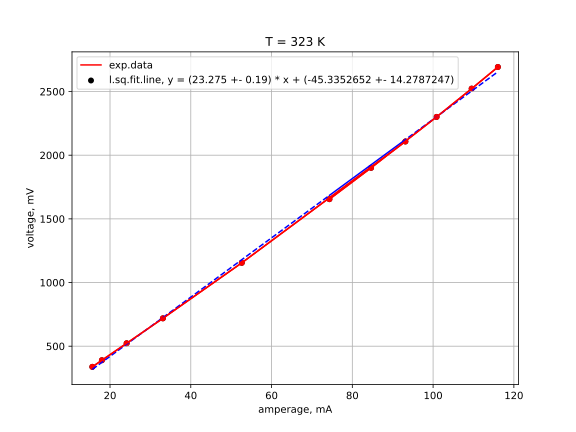
\includegraphics[width=8cm,height=7cm]{physlabwork_11week_3n.png}}
 \ffigbox[\FBwidth]{\caption{не мои данные}\label{fig:Graph_4}}%
         {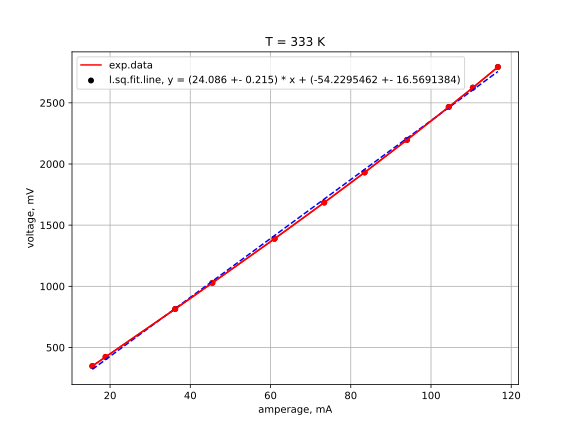
\includegraphics[width=8cm,height=7cm]{physlabwork_11week_4n.png}}         
\end{floatrow}
\end{figure}

\thisfloatsetup{floatrowsep=mysep}	
\begin{figure}[h!]
\begin{floatrow}
 \ffigbox[\FBwidth]{\caption{не мои данные}\label{fig:Graph_5}}%
         {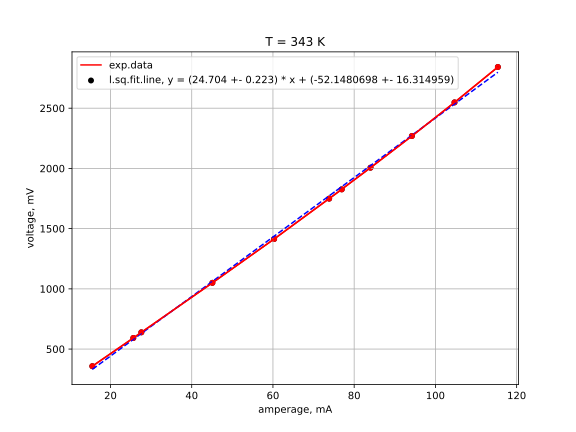
\includegraphics[width=8cm,height=7cm]{physlabwork_11week_5n.png}}     
\end{floatrow}
\end{figure}
\restoregeometry

\newgeometry{bottom=2cm, left=1cm, right=1cm, top=1.5cm}	
\thisfloatsetup{floatrowsep=mysep}	
\begin{figure}[h!]
\begin{floatrow}
 \ffigbox[\FBwidth]{\caption{не мои данные}\label{fig:Graph_1}}%
         {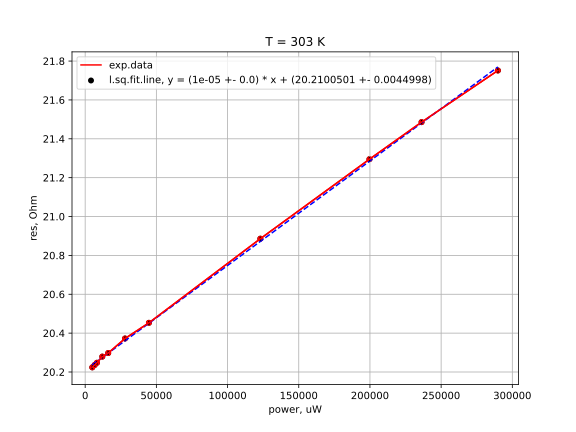
\includegraphics[width=8cm,height=7cm]{physlabwork_11week_1RQn.png}}
 \ffigbox[\FBwidth]{\caption{не мои данные}\label{fig:Graph_2}}%
         {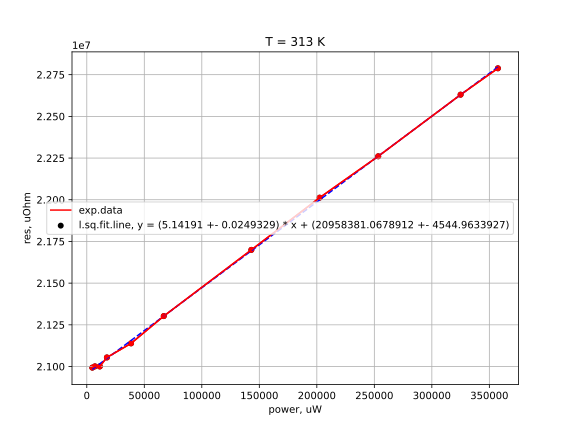
\includegraphics[width=8cm,height=7cm]{physlabwork_11week_2RQn.png}}         
\end{floatrow}
\end{figure}

\thisfloatsetup{floatrowsep=mysep}	
\begin{figure}[h!]
\begin{floatrow}
 \ffigbox[\FBwidth]{\caption{не мои данные}\label{fig:Graph_3}}%
         {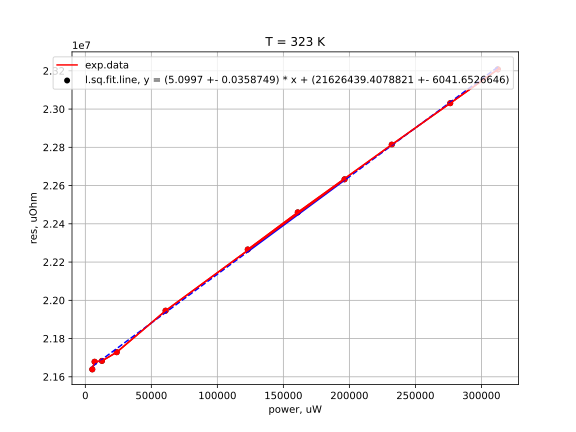
\includegraphics[width=8cm,height=7cm]{physlabwork_11week_3RQn.png}}
 \ffigbox[\FBwidth]{\caption{не мои данные}\label{fig:Graph_4}}%
         {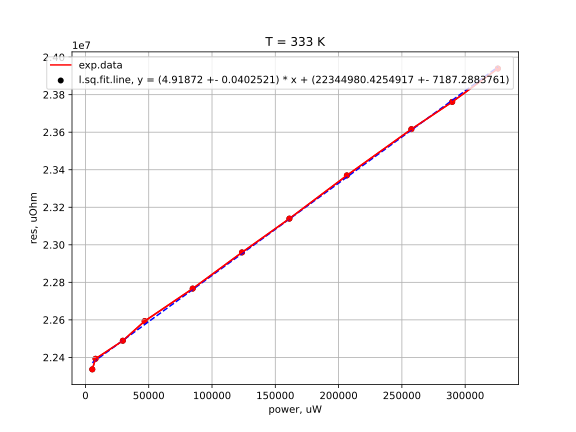
\includegraphics[width=8cm,height=7cm]{physlabwork_11week_4RQn.png}}         
\end{floatrow}
\end{figure}

\thisfloatsetup{floatrowsep=mysep}	
\begin{figure}[h!]
\begin{floatrow}
 \ffigbox[\FBwidth]{\caption{не мои данные}\label{fig:Graph_5}}%
         {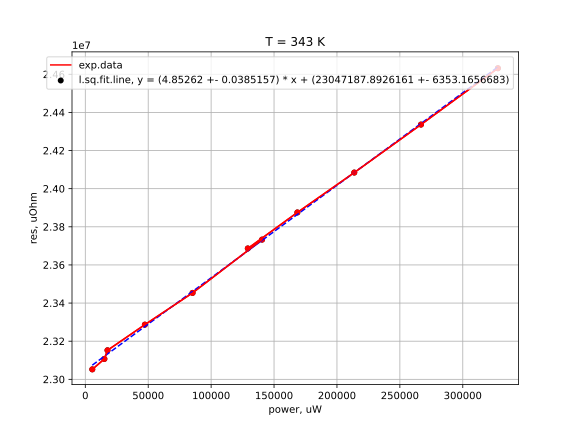
\includegraphics[width=8cm,height=7cm]{physlabwork_11week_5RQn.png}}     
\end{floatrow}
\end{figure}
\restoregeometry

\thisfloatsetup{floatrowsep=mysep}	
\begin{figure}[h!]
\begin{floatrow}
 \ffigbox[\FBwidth]{\caption{}\label{fig:Graph_5}}%
         {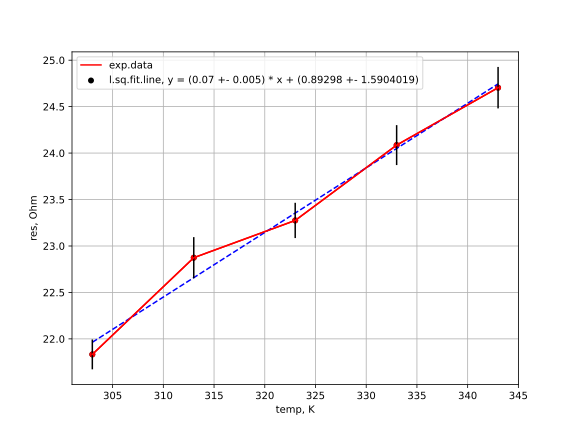
\includegraphics[width=12cm,height=10.5cm]{physlabwork_11week_7RT.png}}     
\end{floatrow}
\end{figure}

\thisfloatsetup{floatrowsep=mysep}	
\begin{figure}[h!]
\begin{floatrow}
 \ffigbox[\FBwidth]{\caption{}\label{fig:Graph_5}}%
         {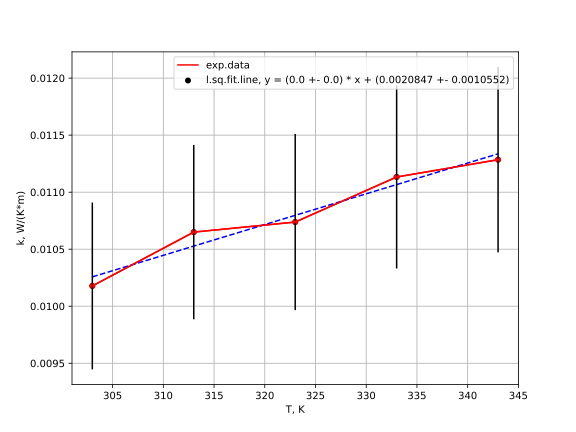
\includegraphics[width=12cm,height=10.5cm]{physlabwork_11week_8kT.png}}     
\end{floatrow}
\end{figure}

\thisfloatsetup{floatrowsep=mysep}	
\begin{figure}[h!]
\begin{floatrow}
 \ffigbox[\FBwidth]{\caption{}\label{fig:Graph_5}}%
         {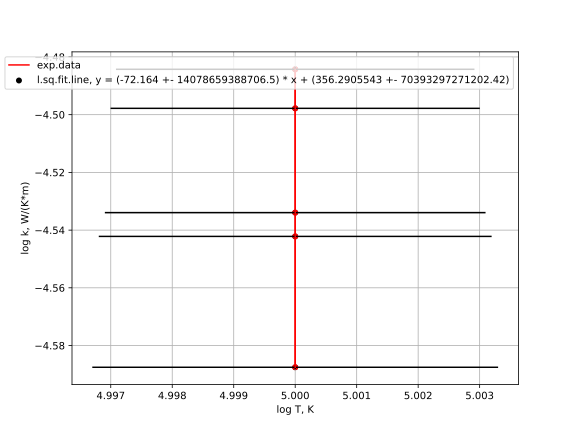
\includegraphics[width=12cm,height=10.5cm]{physlabwork_11week_9logklogT.png}}     
\end{floatrow}
\end{figure}

\section{Обсуждение результатов}
\begin{table}[H]
\caption{}
\label{tabular:timesandtenses}
\begin{center}
\begin{tabular}{ccc}
T, K & k, W/(K*m) & error, W/(K*m)\\
303 & 0.0101780189150949 & 0.000731561164255305\\
313 & 0.0106501312802353 & 0.000764359799245164\\
323 & 0.0107382819638714 & 0.000772627109145082\\
333 & 0.0111333876559664 & 0.000802406637818782\\
343 & 0.0112850411800542 & 0.000813025645850026\\
\end{tabular}
\end{center}
\end{table}
\section{Заключение}

\thisfloatsetup{floatrowsep=mysep}	
\begin{figure}[h!]
\begin{floatrow}
 \ffigbox[\FBwidth]{\caption{}\label{fig:Graph_5}}%
         {\includegraphics[width=6cm,height=4.5cm]{lgh.png}}     
\end{floatrow}
\end{figure}

\end{document}
